\documentclass[11pt,letterpaper]{article}
\usepackage{naaclhlt2010}
\usepackage{times}
\usepackage{latexsym}
\usepackage{url}
\usepackage{graphicx}
\usepackage{rotating}
\usepackage{multirow}
\usepackage{float}
\usepackage{textcomp}
\usepackage{enumerate}
\setlength\titlebox{6.5cm}
%\renewcommand{\baselinestretch}{0.96}


\title{Faster Intersection Via Vector Trees}

\author{
	Adam Gerber \\
	{\tt adam.gerber@jhu.edu}\\
	Johns Hopkins University\\
	3400 North Charles Street \\
	Baltimore, MD 21210, USA\\
	\And 
	{Juri Ganitkevitch} \\
	{\tt j.ganitkevitch@jhu.edu}\\
	Johns Hopkins University\\
	3400 North Charles Street \\
	Baltimore, MD 21210, USA
}

\begin{document}
\maketitle

\begin{abstract}
This paper implements and extends a theoretical framework
for set intersection, developed earlier.  This theoretical framework is
implemented by means of a tree structure called a VectorTree, which
is explained here.  This approach is especially effective
in dealing with sparsity and locality, while maintaining
state of the art performance for dense sets over small ranges.
Here, worst-case scenarios are resolved by introducing
additional data structures which provide insight into the
distributional characteristics of the descendants of each node.
\end{abstract}

%%%%%%%%%%
% Introduction
%%%%%%%%%%

\section{Introduction}
For two sets $A$ and $B$, the set intersection problem consists of
finding the set that contains all elements of $A$ that also appear in $B$,
but no other elements. 

Formally: 
\[x \in A \cap B \iff x \in A \land x \in B\]

\paragraph{}
This definition can be generalized to the intersection of an arbitrary,
nonempty collection of sets. If $M$ is a nonempty set whose elements
are themselves sets, then $x$ is an element of the intersection of $M$,
 if and only if, for every element $A$ of $M$, $x$ is and element of $A$.

Formally:
\[ x \in \cap M \iff \forall A \in M, x \in A\]

\paragraph{}
Many approaches cast intersection as a search problem, modifying familiar
search algorithms to find the common elements in all sets.  Common strategies
exploit disparities in sizes of sets, asymmetries in the distributional characteristics,
and statistics gathered during the lifetime of a set.

\paragraph{}
Many authors consider the intersection problem for ordered sets isomorphic
to the intersection for sets in general.  Further, it is almost universally assumed
that members are of integer type.

\paragraph{}
An early approach to this problem, Hwang, et al \cite{hwang:10},
minimizes searching by linearly searching for each element from a smaller set
in a larger set. More recently, Demaine et al. \cite{338634} proposed an algorithm
which they called Adaptive, which searches for an element of a particular set 
within all other sets using a combination of ``galloping search'' and binary search.
Barbay, et al \cite{1564507} introduced a variant of the Adaptive algorithm,
called Sequential, which cycles through the sets, ``performing one entire
gallop search at a time in each (as opposed to a single galloping step
in Adaptive).''

\paragraph{}
One of the most recent algorithms is due to Baeza-Yates \cite{BY:03}.
This algorithm obtains the median element of the smaller set and attempts
to locate that value within the larger set, dividing the problem into
two sub-problems for each median element, each of which is solved recursively.
Although much of the work in intersection is concerned with search,
Udamchaiporn et al. propose a new approach to the intersection of sorted sets
using a comparison-and-elimination approach that is ``search free''; this method
is described in Section 2.

\paragraph{}
Here, we implement an intersection strategy previously proposed,
which represents the ordered sets by multi-bit offsets, organized hierarchically,
as in a search tree.  This structure gives rise to an efficient intersection procedure
which is described below.

The rest of the paper is organized as follows: related works
are described in Section 2, the algorithm and associated data structures are
described in Section 3, significant cases are discussed in Section 4, future work is
discussed in Section 5, and the conclusion in Section 6.


%%%%%%%%%%
% Related Work
%%%%%%%%%%

\section{Related Work}
Below, we discuss several approaches to the intersection problem that
were relevant to the theoretical framework, which, here, is implemented
and extended.

\paragraph{}
Demain, et al. proposed the Adaptive algorithm which attempts to
match elements using a combination of ``galloping search'' and binary
search.  This algorithm performs the so-called ``gallop'' in parallel through all
the sets from both the ``low side'' and ``high side'' to find eliminators
(elements potentially in the intersection).  According to Demain,
``Galloping consists of doubling the jump in position each iteration,
until it overshoots the current eliminator which will be on the low side.
Upon overshooting, the other parallel processes pause while the overshooter
does a binary search to find the largest eliminatable element and chooses
the next higher element as the new eliminator.``
Adapting to numerous sets of data proved hazardous
to its complexity however.  Barbay, et al.'s Sequential approach is similar,
except for its use of the galloping search as described above, and performs
fewer comparisons than the Adaptive algorithm on average.
	
\paragraph{}
The Baeza-Yates algorithm finds the median element of the smaller of
two ordered sets and uses a binary search to locate the value in the larger set.
If the element is found in the larger set, it is added to the intersection set.
This algorithm then recursively solves the equivalent sub-problem for each
pair of subsets. 

\paragraph{}
The Search-Free algorithm described by Udomchaiporn, et al. takes a different
approach to the intersection problem.  For each ordered set, they identify the
maximal element among the $m$ sets' lowest values and the minimal element
among the $m$ sets' highest values, checking for matches while iteratively
pruning all other sets of members which fall outside of this range, terminating
when a set becomes empty.  This process proceeds in linear time with
the size of the non-matching elements.

\paragraph{}
These approaches all have linear average-case time complexity, and also have
best-case scenarios that may be constant time for degenerate cases or for
very idiosyncratic datasets.  Nevertheless, the sets are represented sequentially
and so are unable to capture the distributional properties of the data.  The
theoretical framework built upon here leverages a structured but tractable
representation of the state space as well as the ability to process large ranges of
data with great efficiency.

%%%%%%%%%%
% Method
%%%%%%%%%%

\section{Method}

\subsection{Context}
While many authors consider the intersection problem in the abstract setting,
we propose an architecture within a component framework, for utilization by
any application, especially solvers such as Prolog or database management
systems (DBMS), such as MySQL.

\paragraph{}
After presenting the original Vector Tree framework in the abstract, we present 
the algorithm fully integrated as a Java package, accessible to all interested parties.

\paragraph{}
The package provides a means of representing ordered sets, which is abstracted
away from the user.  It presents an interface for adding and removing records,
and for executing the intersection, which provides access to this potentially very
large set by means of an iterator, provides the requester with those values in the
intersection (or, if it is preferred, the records to which those keys belong, as may
be useful in the context of a DBMS).

\paragraph{}
A simple example of this would be a query on two tables to find all products that
have a coupon, as in Figure \ref{fig:db-join}. In this case, the algorithm would return
an iterator either (1) over {\tt pid} values within the intersection or (2) over rows,
which correspond to records.  This distinction is determined by the requester.

\begin{figure}[t]
\center
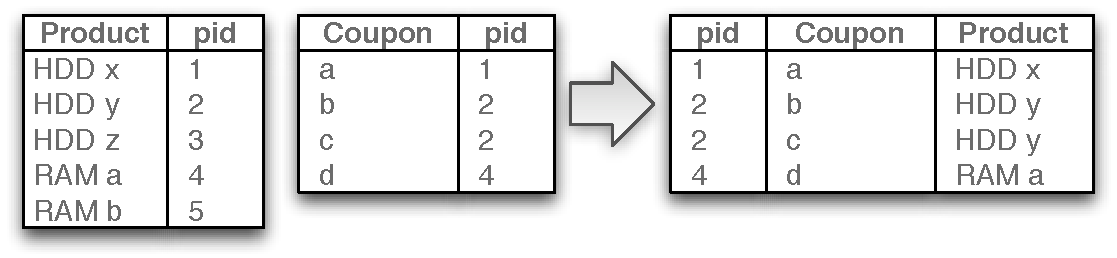
\includegraphics[width=0.98\linewidth]{db-join.pdf}
\caption{A simple database join.}
\label{fig:db-join}
\end{figure}


\subsection{Definitions}

The Vector Tree framework introduce a tree structure for storing
$m$-bit integer keys, where $m$ must be of the form $m=Di$,
where $i=2^n$ for some small integers $D$ and $n$.

\paragraph{}
For example, to represent 32-bit integers, one such assignment
would be $n=3$ and $D=4$, with $i=2^n=8$.  From the definition of
$m$, it is clear that it is possible to segment every $m$-bit integer
into $d$ contiguous $i$-bit sequences.

\paragraph{}
We will use the notation $sig_i(key, j)$ to denote a $key$'s
$j^{th}$ most significant $i$-bit sequence.  In other words,
for any key $k_q$ in the range $2^{Di}$, the following serves as
an identity, where $\oplus$ is the append operator:

\[ k_q = sig_i(k_q, 0) \oplus sig_i(k_q, 1) \oplus ... \oplus sig_i(k_q, D-1) \]

\paragraph{}
Formally, a Vector Tree $T$ consists of a hash table called
{\tt nodes}, which maps bitvectors to a finite set of tuples, each
corresponding to a node in the tree.  These tuples are of the form $(c, m, p)$,
where $c \in [0, 2^{2^i}]$ indicates the current bit configuration,
$m$ the number of leaf nodes (equivalent to the number of unique
keys that have been inserted into that node's subtrees), and $p$
is the total number of non-leaf nodes beneath that node.  A Vector
Tree has an additional hash table called {\tt registrants}, which maps
full keys to lists of objects that are associated with them.

\paragraph{}
The Vector Tree support several operations:

\begin{itemize}
	\item Insertion
	\item Deletion
	\item Intersection
		\begin{itemize}
			\item BitwiseIntersect
			\item SurvivorMap
		\end{itemize}
\end{itemize}

\subsubsection{Similar Structures}
Similarities can be drawn to a van Emde Boas tree \cite{wiki:001},
although without the root-size reduction in range at each level, or to a suffix tree, in
which the bit-vectors are symbols in alphabet of size $2^i$.

\begin{figure}[t]
	\center
	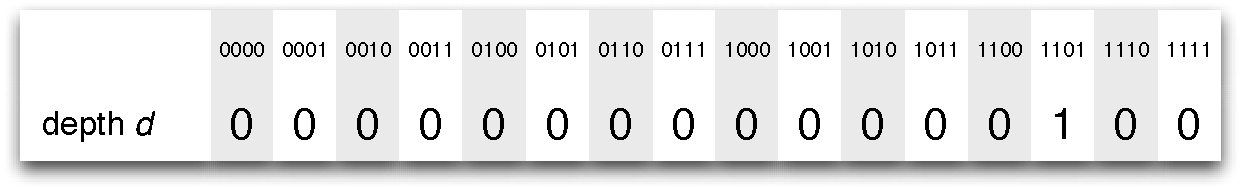
\includegraphics[width=0.98\linewidth]{example-vector.pdf}
	\caption{An example bit-vector for $i=4$.}
	\label{fig:example-vector}
\end{figure}

\subsection{Encoding}
For a Vector Tree $T$ over the universe $0$ to $2^m - 1$, the root node
encodes $sig_i(key, 0)$ in a bit-vector of length $2^i$,
with each bit corresponding to one of the $2^i$ combinations possible
among $i$ bits.  For example, where $i=4$, the 4-bit sequence {\tt 0000}
would correspond to the first of the vector's 16 elements.  This is illustrated
in Figure \ref{fig:example-vector}.

\paragraph{}
Just as the root node, with depth 0, encodes the sequence $sig_i(key, 0)$,
nodes at depth 1 encode the sequence $sig_i(key, 1)$, and,
in general, nodes at depth $d$ encode $sig_i(key, d)$.  Nodes at the
same depth, but which do not share a parent encode the same $i$-bits
of the key, but they necessarily differ in the bit sequence which precedes
the sequence they encode.  This preceding sequence is called the node's
bit prefix.

\paragraph{}
An ``on" ({\tt 1}) bit in the root node's bit-vector guarantees the existence
of at least one key whose first $i$ bits match the $i$-bit combination
indicated by the bit-vector.  Correspondingly, an ``off" bit ({\tt 0}) indicates
the absence of any such element.  For example, in the case $i=4$,
if the root node's bit-vector is {\tt 1000000000000001}, then the tree is
guaranteed to contain at least one key $k_1$ with $sig_4(k_1, 0) = {\tt 0000}$
and at least one key $k_2$ with $sig_4(k_2, 0)={\tt 1111}$.  Similarly, a node's
bitvector will never contain only zeros, because this would indicate there are
no values in this range, in which case the node does not exist (it may be created
in a subsequent {\tt Insert} operation).

\subsubsection{Node Hierarchy}
Unlike typical tree structures, in which a parent node contains
pointers to its child nodes, nodes in the Vector Tree, parents and children have no
direct connection. Instead, the hash table {\tt Nodes} is used for random-access to any
node in tree.  This is possible because every node in the tree (and, more strongly,
every possible node) can be uniquely specified by its bit-vector.  For example, assuming
$i=4$, the bit-prefix {\tt 00000000} specifies the left-most node at a depth of 2.  The
empty bit-prefix specifies the root (which is the initial position and has no prefix).

\subsubsection{Leaves}
Unlike other nodes, a materialized leaf node contains a table, which, for all keys
in the node's $2^i$ value range, maps each key to a list of object references.
This allows for the constant-time recovery of all associated objects, for example,
the record of which this key is a column-value or the class instance of which this
key is a member.



%%%%%%%%%%
% Operations
%%%%%%%%%%

\subsection{Operations}

\begin{figure*}[t]
	\center
	\fbox{
		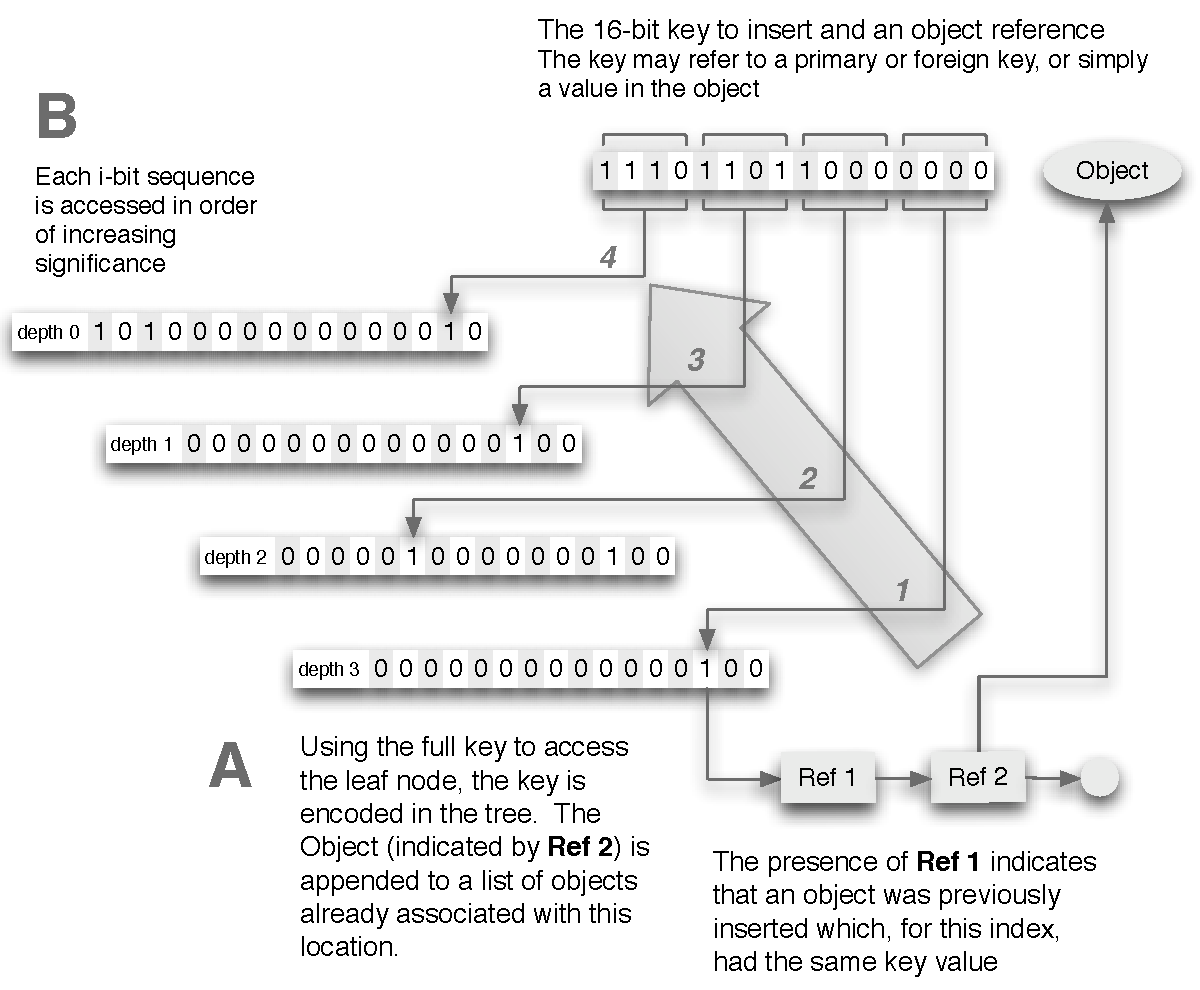
\includegraphics[width=0.98\linewidth]{insertion-05.pdf}}
\caption{Insertion of a key.}
\label{fig:insertion-diagram}
\end{figure*}

\subsubsection{Insertion}
Figure \ref{fig:insertion-diagram} outlines the insertion of the key
{\tt 111011010000000} along with the object of which this key
is a component.  As described in A, the full key is used with {\tt nodes}
to access the proper leaf node, and a reference to the object is
added to this key's list in {\tt registrants}.

\paragraph{}
If the corresponding bit is already on, then the insertion operation
concludes. If the bit is off, then it is flipped, and the node's member count
is incremented.  Then, the leaf node's parent is accessed (also via
{\tt nodes} by splicing off the least-significant $i$-bits from the key.
It may be the case that this node does not yet exist, in which case, 
an empty node is initialized.  In either case, the parent's progeny
count is incremented and the bit corresponding to the leaf node is queried.

\paragraph{}
If the bit is already on, then the process
terminates; otherwise, the bit is flipped and this process advances
up the tree, terminating after reaching (and, if necessary, updating)
the root node.

\subsubsection{Deletion}
Deletion requires both a key and an object as parameters, as multiple
objects may be registered to the same key.  The full bit-sequence of the
key is used with {\tt nodes} to obtain its containing leaf node.
The list of objects registered to the key is obtained via {\tt registrants}
and is scanned for a reference to an object that matches the object parameter.
If a match is found, then the reference is removed.  If a removal occurred,
then the list is queried to determine whether any objects remain registered
to this key, if not, the bit corresponding to the key is turned off, and the
member count for the node is decremented.

\paragraph{}
If this update results in a member count of zero, then the node is
decommissioned and the tree's node hash for this key is set to null.

\paragraph{}
If the member count was decremented, then the parent node is loaded
and its member count is decremented.  If the child node was decommissioned,
then the bit corresponding to that child is turned off and the parent node's
progeny count is decremented.  As a bit change occurred, the vector is passed
as a parameter to {\tt SurvivorMap}; if the mapping function returns an
empty list, then the node has no children remaining, and so it too
is decommissioned.  The process repeats for each parent node, up to and
including the root node.

\subsection{Intersection Algorithm}
\subsubsection{{\tt Bitwise Intersection}}
This method takes, as input, $m$ vectors, efficiently perform
a bitwise {\tt AND} operation, and returns the result.
This operation is constant in the size of the vector and can also be
constant in the size of $m$, however, in the worst case, is $O$(lg $m$).

\subsubsection{{\tt SurvivorMap}}
This method takes, as input a vector of length $2^i$ and, in constant-time,
returns a list of the ``on'' bits, in their $i$-bit encoding.  For example,
for $i=4$, the call {\tt SurvivorMap}({\tt 1100000010000001}) would
return the following:
\[ {\tt [0000,0001,1000,1111]}\]

\paragraph{}
Constant-time (as opposed to time proportional to the size of the input)
is achieved by precomputing the entire mapping of $2^{2^i}$ configurations
of $2^i$.  For example, for $i=4$, node vectors must be of length $2^4=16$,
which means this method must store a range of $2^16=65536$ values.

\paragraph{}
An example of this can be seen in B and C in Figure \ref{fig:intersection-diagram}.


\begin{figure*}[t]
\center{\fbox{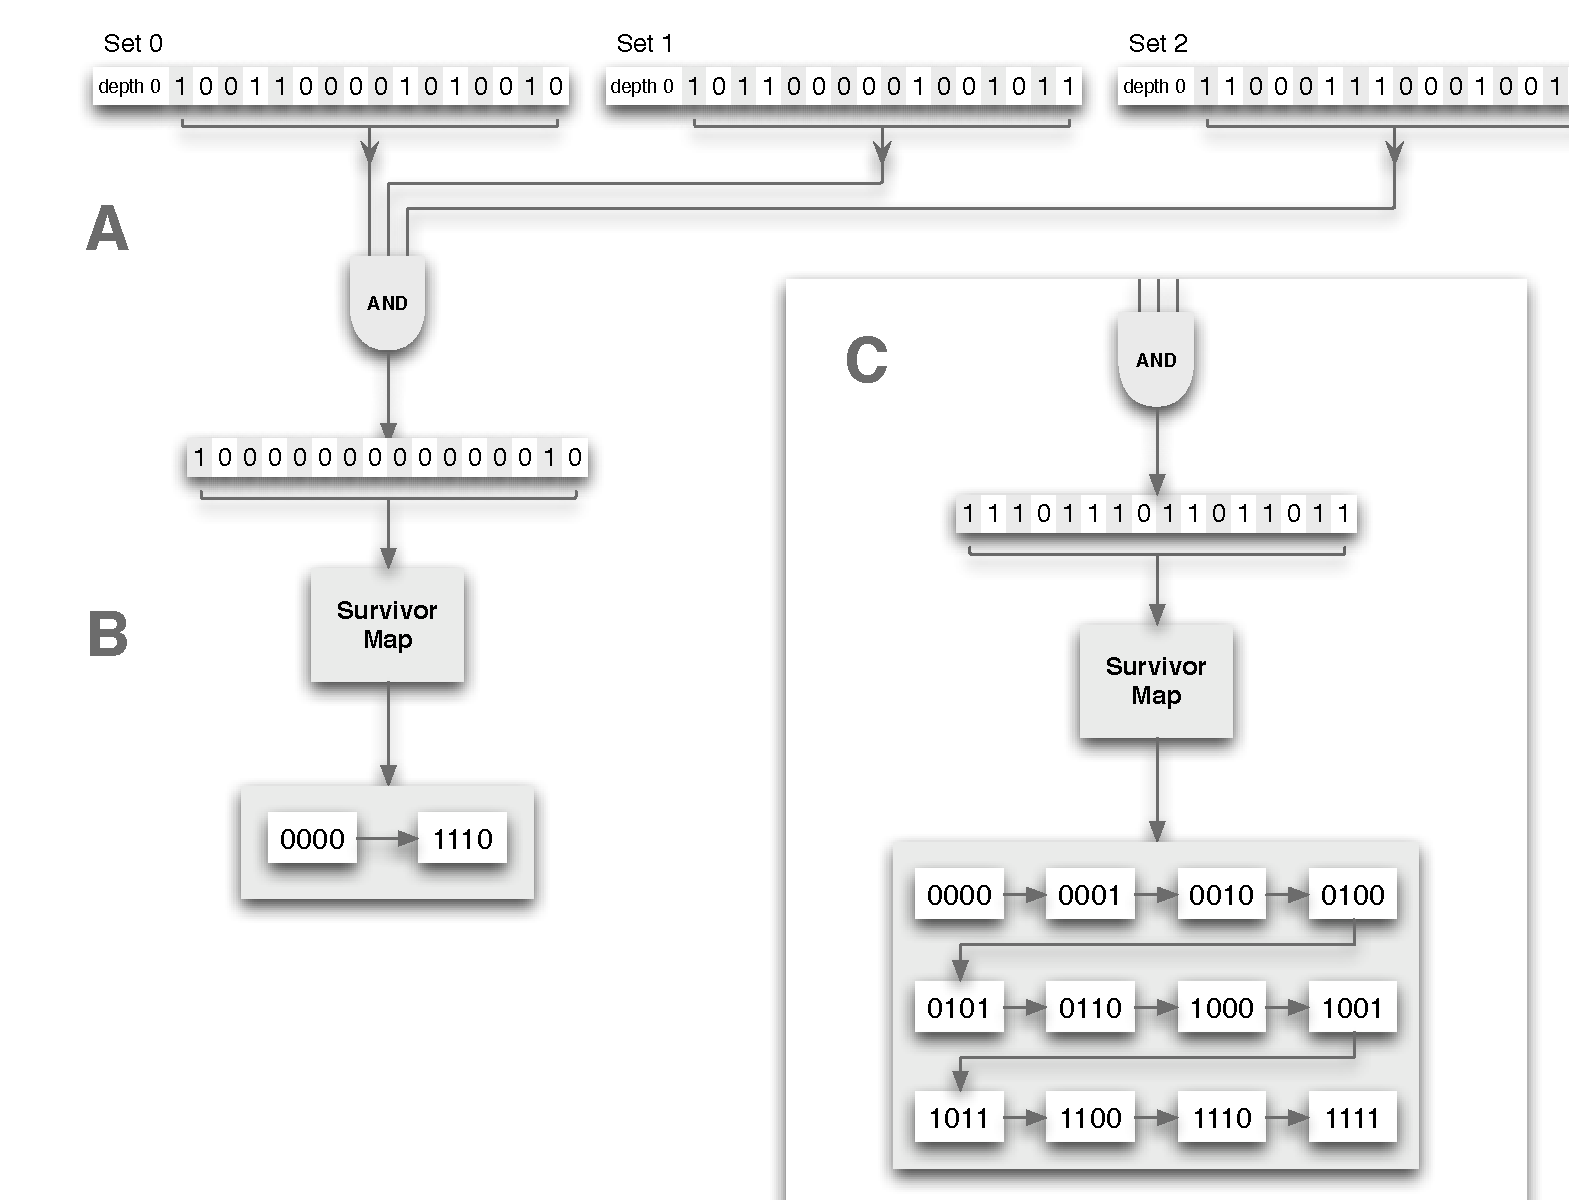
\includegraphics[width=0.98\linewidth]{intersection-06.pdf}}}
\caption{Initial step in the intersection of 3 sets}
\label{fig:intersection-diagram}
\end{figure*}

\subsubsection{Intersection}

The intersection procedure begins by initializing an iterator and a queue.
The iterator will read from the queue whenever a caller requests an
element of the intersection.  The queue is the structure onto which elements
in the intersection will be pushed.

\subparagraph{}
The process continues by obtaining the bit-vector at the root node
of each of the $m$ sets involved in the intersection and passing them to the
method {\tt BitwiseIntersection}, which produces the intersection of the bit-vectors.
Rather than scan the bit-vector for ``on'' bits, we pass the result as a parameter
to the method {\tt SurvivorMap}, which returns a list of indices that correspond
to the ``on'' bits in the bitwise-intersection parameter and, more importantly, to
the surviving subtrees.  This process occurs in constant time for each node.
It should be noted that intersection is not guaranteed at this stage; the only
assurance is that all sets contain members in the indicated range.

\subparagraph{}
If this list is empty, then we move to the parent of the
current node; however, if the current node is the root node, then the operation
terminates.
If the list is not empty, then each index is used to create a key to access the bit-vectors
at next search location.  To create the key, the index is appended to the the bit-prefix
of the current location.  For each of the $m$ sets, the key is then used to access
the surviving node and obtain its bit-vector.  The process repeats as before, until
a leaf node is reached.  A depiction of this initial iteration can be seen in
Figure \ref{fig:intersection-diagram}.

\subparagraph{}
In the leaf node, the procedure is only slightly different.  Just as before
the bit-vectors are obtained from each of the $m$ sets.  Here, too, they
are passed to {\tt BitwiseIntersection}, which returns a bit-vector; however
this bit-vector does not indicate common ranges as before, but, instead,
 actual matching keys.  We nevertheless want to leverage {\tt SurvivorMap}'s
constant-time conversion of vector to list, but we will handle the resulting list differently.

\subparagraph{}
First, we will push onto the queue a metadata object, then we will push the 
entire list of indices returned by {\tt SurvivorMap}.  The metadata object, 
interpretable by the iterator, will (1) provide access to {\tt Registrants} so that
the references or records associated with a key can be accessed over all sets
(for example, allowing them to be combined, as in a join operation, and for 
external access to the potentially numerous objects sharing a key), and
(2) provides the iterator with the bit-prefix of the current location.  The bit-prefix
provides the iterator with sufficient information to recover the matching key
at time of user request, allowing us to remain in constant-time for each node.

% Begin traversing from root Among all m trees, does any have
% memberCount of q, where q is a parameter indicating the threshold
% for direct-value comparison if so, find the tree least likely to
% contain a match in that range.  fewest members

\section{Bloom Filter Guarding}

While our method presents an efficient approach to multi-set
intersection, there are cases in which an unfortunate distribution of
the data causes the algorithm to explore the entire tree only to find
that there are no, or only very few, matches. Consider for instance
sparse, uniformly distributed sets with little overlap. While the
uniformity will for many sets result in a full Vector Tree, the
sparsity entails that only very few of the leaf nodes actually contain
matching keys.

We address this issue by introducing Bloom filters, a probabilistic
data-structure that provides a compact bit-vector representation of
the keys in the sub-tree rooted in each node.

\subsection{Bloom Filters}

A Bloom filter consists of a bit vector of size $m$ and a set of $k$
hash functions $h_1, \ldots, h_k$ that map any object to an integer $1
\ldots m$. To insert an object $o$ into the filter, we compute
$h_i(o)$ for each hash function and set the corresponding bit in the
bit vector to 1. To check whether an object is in the Bloom filter, we
similarly compute the hash indices for each of the $k$ functions and
test whether the corresponding bits are 1. Since the sets of bits set
for different objects can overlap (i.e.\ $h_i(o) = h_j(o')$), querys
to the Bloom filter can result in false positives, however (since a
bit set to 1 it is never flipped back) never in false negatives. 

Bloom filters have been thoroughly studied and bounds on the false
positive rate for a given $m$, expected number $n$ of objects to be
inserted into the filter as well as the optimal $k$ for given $m$ and
$n$ are readily available in the literature.

\subsection{Use of Bloom Filters in the Vector Tree}

We augment the Vector Tree structure by adding a Bloom filter to each
node in the tree. Each Bloom filter contains the keys in the subtree
rooted at its respective node. Furthermore, for a given depth $d$, all
Bloom filters are of the same size and employ the same set of hash
functions. This setup makes the resulting bit vectors comparable
across two or more Vector Trees\footnote{Obviously, we only compare
  the Bloom filters of nodes that govern the same key prefix.},
enabling us to use the Bloom filters to obtain information useful in
the tree intersection process.

When intersecting a set of nodes $n_i$, we first intersect their Bloom
filters $b_i$ by computing a bit vector $b = \bigwedge_i b_i$ through
bit-wise intersection of the $b_i$. Since the Bloom filters are of
equal size and use the same set of hash functions, a key is present in
all the $b_i$ will be present in $b$. Conversely, if $b$ is all zeros
we are guaranteed that the $b_i$ do not contain any common
keys. Furthermore the number of ones in $b$, divided by the number of
hash functions, $\frac{|b|_1}{k}$, gives us an estimate (and upper
bound) on the number of common elements in the subtrees. The precision
of this estimate depends on the false positive rate of the Bloom
filters

This information can be used to avoid descend into subtrees that
exhibit identical structure, yet do not contain matching keys. The
deeper the node is in the Vector Tree, the smaller the range of
potential keys it covers and the smaller the Bloom filter required to
maintain an acceptable false positive rate. Additionally, we vary the
hash function sets used for each depth level, creating a more diverse
set of Bloom filters that are overall less likely to produce false
positives over the same data.

\section{Analysis}

While describing the asymptotic time complexity of many algorithms is useful,
in the case of the intersection problem even the most naive methods will
approach linear time.  For this reason, we present a number of cases and
compare how the Vector Tree algorithm performs in comparison to the Search-Free
algorithm and the Baeza-Yates algorithm.

\subsection{Case 1}
Consider the case of $m$ sets over the range of $0$ to $2^{Di} - 1$,
with $r$ regions of dense keys (with an average of $k$ keys per region),
sparsely distributed over the key range.  Let $P$ represent the set of
regions that will be in the intersection set and $Q$ be the set of all those
regions that will be pruned (i.e. not in the intersection).

\paragraph{}
For all regions in $P$, both the Search-Free algorithm and the
Baeza-Yates algorithm would require an average of $km$ comparisons
per region.  However, the Vector Tree approach would require, in the
worst case, $\frac{(2^i)^{X+1}}{2^i-1}$ comparisons where $X=\frac{k}{2^i}$.
This is because at every level $d$ of the tree, a maximum of $2^{id}$
comparisons are performed.  As the algorithm recurses down the tree,
intersections are performed successively, eliminating unnecessary branches
until it reaches a leaf node.  For each leaf, there are only $2^i$ candidates for
the intersection set; determining the remaining candidates is a constant-time
operation at the leaf level, regardless of the number of elements added to the
intersection set

For all regions in $Q$, the Search-Free algorithm would still
perform $km$ operations per region $r$ (each key in each set must
be set to null), while the Baeza-Yates algorithm would do close to $km$
comparisons over all regions. In this case, the Vector Tree algorithm
would perform a maximum of $\frac{(2^i)^{X+1}}{2^i-1}$ comparisons
where $X=\frac{k}{2^i}$ to prune that part of the tree. In practice, it is
likely to perform significantly fewer comparisons for regions in $Q$ because
large blocks of elements would be eliminated closer to the root node.
Because of this, on the order of $2^i$ comparisons are avoided, speeding
up the intersection accordingly. 

\paragraph{}
Wasteful comparisons are nevertheless made.  The Search-Free algorithm
performs approximately $km$ comparisons, as does the Baeza-Yates
algorithm, while the Vector Tree performs $\frac{(2^i)^{X+1}}{2^i-1}$
comparisons where $X=\frac{k}{2^i}$. In cases of large $r$ in both $P$
and $Q$, the Vector Tree prunes the regions of Q in the same time,
while the other algorithms (with the exception of those implementing gallop
search) are limited to examining individual keys.  In $P$, the Vector Tree
performs comparisons of $2^i$ elements for every single element compared
in the other approaches.

\section{Experimental Results}

The space over which we aim to obtain performance results is a highly
parametrized one. We conduct our experiments on synthetic data, i.e.\
randomly generated sets of keys. This approach provides us with good
control over the nature of the task we evaluate on. We describe the
data generation procedure in the following sub-section and then
proceed to present a selection of performance statistics we obtained
in our experiments.

\subsection{Data Generation}

We focus on two factors that we deem important when conducting
multi-set intersections: data sparsity and data set overlap. While in
real-world applications keys can't generally be assumed to be
uniformly distributed, we generate our synthetic key sets from uniform
distributions\footnote{In fact, we have implemented a method to
  generate more complex key distributions by combining multiple local
  uniform or normal distribution, leading to locally denser key
  sets. However, we did not use this data in our experiments.}. The
data generation process works as follows: we first determine the
number $n$ and size $m$ of key sets to intersect, as well as the
sparsity ratio -- defined as $\sigma =
\frac{\mathit{keys~in~set}}{\mathit{keys~in~scope}}$, where the scope
is the overall set of keys we draw from uniformly. The size of the
scope is determined by reversing the rationale and given by
$\frac{m}{\sigma}$. We then generate a root key set by uniformly
drawing $m$ keys from a set of $\frac{m}{\sigma}$. Next, we set an
overlap factor $\omega =
\frac{\mathit{keys~shared~with~root~set}}{\mathit{keys~in~set}}$. The
remainder of the sets are then constructed by uniformly drawing from
the root set until $\omega$ is fulfilled and padded with keys drawn
uniformly from the set of all possible integers.

\subsection{Experiments}

Here, we present performance results for multiset intersections using
the Vector Tree structure, with and without the Bloom filter
augmentation. Aside from the number, size, sparisity and overlap of
the data sets, we also investigate two parameters that affect the
Bloom filters themselves. 

As mentioned earlier, Bloom filters rely on an estimate of the number
of keys they will hold to parametrize optimally. In our setup, this
estimate is very crude: we simply use the maximum number of keys that
a particular node \emph{could} hold. I.e.\ the set of all integers
($2^{32}$ in Java) at the root node etc. Clearly, in a more realistic
setting this estimate could be bounded by the total number of objects
in the database and computed from more sophisticated statistics. The
result of using an estimate this crude is, that a Bloom filter that
were able to hold this many object would itself be unreasonably
large. While attemping to partially amend this problem by making the
Bloom filter as large as memory permits may be an option it turns out
to be a bad choice for two reasons: firstly, the resulting bit vectors
are very large and therefore relatively costly to intersect. Secondly,
decisions made at nodes close to the tree root (for which we are
facing this problem) are of very low granularity: eliminations here
are quite unlikely. This results in a trade-off: instead of querying
Bloom filter


\section{Future Work}
\subsection{Greater Bit Length}
In practice, $i=4$ is the highest feasible bit-length that allows the constant-time
strategies we employed here.  This is because {\tt SurvivorMap} must encode
all $2^{2^i}$ combinations of vector combinations.  With $i=4$, this means
65536 keys, but for $i=8$, this would require $2^{2^8}=2^{256}=1.1579\times10^{77}$
keys.  However, there may be intermediate values that are viable.

\subsection{Alternate Encodings}
In this investigation, we used significant-bits as the partition criteria,
however, it may be the case that other encodings have distributional properties
that allow for greater sparsity or dissimilarity between regions.

\subsection{Alternate Encodings}
In this investigation, we used significant-bits as the partition criteria,
however, it may be the case that other encodings have distributional properties
that allow for greater sparsity or dissimilarity between regions.


\section{Conclusion}
We have proposed a set-intersection algorithm that performs well
on average and is frequently able to eliminate very large regions of
the keyspace, as well as exploit both sparsity and data locality.  
This algorithm has an average case time complexity of
$O\left(b^{\frac{k}{b}}\right)$ where $b$ is the size of the bit-vector,
and $k$ is a measure of data sparsity. This algorithm is efficient in almost
all cases and does not suffer any severe performance losses on any one
specific case. There are several improvements were would like to consider
and those are further discussed in Future Work.

\section*{Acknowledgments}
The authors would like to thank Wes Filardo for his time and his insight.

\bibliography{writeup}
\bibliographystyle{plain}

\end{document}


